\StartChapter{Vektoranalysis}

\SubsectionBar{Skalarfeld- und Vektorfeld}
\textVorBox{In einem \ZSFkeyword{Skalarfeld} wird jedem Punkt ein Skalar zugewiesen:}
\begin{formulabox}
    $\displaystyle f:(x,y,z)\to f(x,y,z)$
\end{formulabox}

\textVorBox{In einem \ZSFkeyword{Vektorfeld} wird jedem Punkt ein Vektor zugewiesen:}
\begin{formulabox}
    $\displaystyle \vec f:(x,y,z)\to \vec v(x,y,z)$
\end{formulabox}

Wenn $K$ eine Kurve ist, sodass $\vec v$ an jedem Punkt tangential an $K$ anliegt, dann ist $K$ eine \ZSFkeyword{Feldlinie} des Vektorfeldes.

Zeitunabh\"angige Vektorfelder nennt man \ZSFkeyword{station\"ar} und solche die zeitabh\"angig sind \ZSFkeyword{instation\"ar}.

Wenn $\vec v(\vec r)=c\cdot\vec r$, dann ist $\vec v$ \ZSFkeyword{homogen} und alle Feldlinien sind parallele Geraden.

\SubsectionBar{Differentialoperatoren}
\textVorBox{\ZSFkeyword{Operatoren} wandeln Skalarfelder in Vektorfelder um und umgekehrt:}
\begin{formulabox}
    
\includegraphics[width=\linewidth,keepaspectratio]{graphics/media/vektor_operatoren_schema.png}
\end{formulabox}

\textVorBox{Der Gradient ist bereits bekannt:}
\begin{formulabox}
    $\displaystyle \grad(f)=\begin{pmatrix}f_x\\f_y\\f_z\end{pmatrix}$
\end{formulabox}
\textVorBox{In \ZSFkeyword{Zylinderkoordinaten} $(r,\varphi,z)$ bleibt die Struktur erhalten, die $\varphi$-Komponente erh\"alt jedoch den Vorfaktor $\tfrac{1}{r}$:}
\begin{formulabox}
    $\displaystyle \grad(f)=\begin{pmatrix}f_r\\[2pt]\dfrac{1}{r}\,f_\varphi\\[2pt]f_z\end{pmatrix}
    = f_r\,\vec e_r+\frac{1}{r}\,f_\varphi\,\vec e_\varphi+f_z\,\vec e_z$
\end{formulabox}
\begin{itemize}
    \item F\"ur ein Skalarfeld $f$ ist $\grad(f)$ das zugeh\"orige Vektorfeld, das sogenannte \ZSFkeyword{Gradientenfeld}.
\end{itemize}

\textVorBox{Die \ZSFkeyword{Divergenz} eines Vektorfeldes $\vec v$ gibt an, wie "quellenhaltig" dieses ist und berechnet sich mit:}
\begin{formulabox}
    $\displaystyle \divg\,\vec v
    = \frac{\partial v_1}{\partial x} + \frac{\partial v_2}{\partial y} + \frac{\partial v_3}{\partial z}
    = \vec\nabla\cdot\vec v$
\end{formulabox}
\begin{itemize}
    \item Wenn $\divg\,\vec v=0$, dann ist das Feld \ZSFkeyword{quellenfrei}.
    \item Wenn an einem beliebigen Punkt $P_0$ gilt, dass $\divg\,\vec v(P_0)>0$, dann handelt es sich um eine Quelle.
    \item Wenn an einem beliebigen Punkt $P_0$ gilt, dass $\divg\,\vec v(P_0)<0$, dann handelt es sich um eine Senke.
\end{itemize}

\textVorBox{Die \ZSFkeyword{Rotation} eines Vektorfeldes $\vec v$ gibt an, wie "wirbelig" dieses ist und berechnet sich mit:}
\begin{formulabox}
    $\displaystyle \rot\,\vec v=\vec\nabla\times\vec v
    =\begin{pmatrix}
        v_{3,y}-v_{2,z}\\
        v_{1,z}-v_{3,x}\\
        v_{2,x}-v_{1,y}
    \end{pmatrix}$
\end{formulabox}
\begin{itemize}
    \item Wenn $\rot\,\vec v=\vec 0$, dann ist das Feld \ZSFkeyword{wirbelfrei}.
\end{itemize}

F\"ur ein beliebiges Koordinatensystem $(\xi,\eta,\zeta)$ \"andern sich bei der Berechnung von Gradienten, Divergenzen und der Rotation lediglich die partiellen Ableitungen.

\textVorBox{Der \ZSFkeyword{Laplace Operator} ist f\"ur $f:(x,y,z)\to f(x,y,z)$ und $f:(r,\varphi)\to f(r,\varphi)$ definiert durch:}
\begin{formulabox}
    $\displaystyle \nabla f=\divg(\grad f)=f_{xx}+f_{yy}+f_{zz}$

    $\displaystyle \nabla f=\divg(\grad f)=f_{rr}+\frac{1}{r}f_r+\frac{1}{r^2}f_{\varphi\varphi}$
\end{formulabox}

\textVorBox{Weitere Identit\"aten lauten:}
\begin{formulabox}
    $\displaystyle \divg(\rot\,\vec v)=0$

    $\displaystyle \rot(\grad f)=\vec 0$

    $\displaystyle \divg(f\,\rot\,\vec v)=\grad f\cdot \rot\,\vec v$

    $\displaystyle \divg(f\,\vec v)=f\,\divg\vec v+\grad f\cdot\vec v$
\end{formulabox}

\SubsectionBar{Fl\"achen in Parameterdarstellung}
\textVorBox{Sei $\tilde r(u,v)=(x(u,v),y(u,v),z(u,v))$ die Parametrisierung einer Fl\"ache, dann betr\"agt ihr Normaleneinheitsvektor:}
\begin{formulabox}
    $\displaystyle \vec n(u,v)=\pm\frac{\vec r_u\times\vec r_v}{\left|\vec r_u\times\vec r_v\right|}$
\end{formulabox}
\textNachBox{Je nach Parametrisierung muss das Vorzeichen ge\"andert werden.
$\vec r_u$ bedeutet, dass jeder Vektoreintrag nach $u$ abgeleitet ist.}

\textVorBox{Die Gesamtfl\"ache einer parametrierten Fl\"ache $B$ lautet:}
\begin{formulabox}
    $\displaystyle A_B=\iint_B \left|\vec r_u\times\vec r_v\right|\,du\,dv$
\end{formulabox}

\textVorBox{Das von zwei Fl\"achen $B$ und $f$ umschlossene Volumen betr\"agt:}
\begin{formulabox}
    $\displaystyle V_B=\iint_B f(\tilde r(u,v))\left|\vec r_u\times\vec r_v\right|\,du\,dv$
\end{formulabox}

\textVorBox{H\"alt man einen der Parameter fest und variiert den anderen, so erh\"alt man eine Parameterlinie.
Sei $K$ eine parametrisierte Raumkurve $\tilde r(u)=(x(u),y(u),z(u))$, so ist die Tangentialfl\"ache an $K$:}
\begin{formulabox}
    $\displaystyle \tilde r(u,v)=\vec s(u)+v\vec s\,'(u)$
\end{formulabox}

\SubsectionBar{Fluss}
\textVorBox{Der \ZSFkeyword{Fluss} $\Phi$ beschreibt, wie viel Vektorfeld $\vec v$ durch eine Oberfl\"ache $S$ fliesst:}
\begin{formulabox}
    $\displaystyle \Phi=\iint_S \vec v\cdot\vec n\,dO$
\end{formulabox}
\textNachBox{wobei $\vec n$ der Fl\"achennormalenvektor ist.}

\textVorBox{Der Fluss durch ein homogenes, ebenes Vektorfeld durch eine ebene Fl\"ache mit Oberfl\"acheninhalt $O$ gilt:}
\begin{formulabox}
    $\displaystyle \Phi=(\vec v\cdot\vec n)\cdot O$
\end{formulabox}

\textVorBox{Ist $\vec v$ mit $\tilde r(u,v)$ parametrisiert, dann gilt:}
\begin{formulabox}
    $\displaystyle \Phi=\iint_B \vec v\cdot\vec n\,dO
    =\iint_B \vec v(\tilde r(u,v))\cdot(\vec r_u\times\vec r_v)\,du\,dv$
\end{formulabox}
\textNachBox{$\pm$ muss dabei so gew\"ahlt werden, dass $\pm\left[\vec r_u\times\vec r_v\right]$ und $\vec n$ in dieselbe Richtung zeigen (falls $\vec n$ meist in Aufgabenstellungen gegeben).}

\textVorBox{Der \ZSFkeyword{Divergenzsatz von Gauss} besagt, dass ein stetig differenzierbares Vektorfeld (Komponenten sind differenzierbar und die Ableitungen stetig) in einem beschr\"ankten Volumen $B\subset D(\vec v)$ mit Rand $\partial B$ von innen nach aussen den Fluss besitzt:}
\begin{formulabox}
    $\displaystyle \Phi=\iint_{\partial B}\vec v\cdot\vec n\,dO=\iiint_B \divg\,\vec v\,dV$
\end{formulabox}
\textNachBox{\ZSFdanger{Achtung:} z.B. nicht anwendbar bei einer Kugel im Ursprung mit $D(\vec v)=\R^3\setminus\{(0,0,0)\}$.}

\textVorBox{F\"ur geschlossene K\"orper mit mehreren Oberfl\"achenst\"ucken (z.B. $S$ und $D$) und Volumen $V$ gilt:}
\begin{formulabox}
    $\displaystyle \iiint_V \divg\,\vec v\,dV=\iint_{S\cup D}\vec v\cdot\vec n\,dO
    =\iint_S \vec v\cdot\vec n\,dO+\iint_D \vec v\cdot\vec n\,dO$
\end{formulabox}
\textNachBox{wobei $\vec n$ jeweils nach aussen zeigt.}

\SubsectionBar{Arbeit}
\textVorBox{Die \ZSFkeyword{Arbeit} $A$ eines ebenen homogenen Vektorfelds $\vec v$ entlang eines Weges $\gamma$ der L\"ange $L$ betr\"agt:}
\begin{formulabox}
    $\displaystyle W=|\vec v|L\cos(\alpha)$
\end{formulabox}
\textNachBox{wobei $\alpha$ der Winkel zwischen $\vec v$ und $\gamma$ ist.}

\textVorBox{In Integralform l\"asst sich diese wie folgt darstellen:}
\begin{formulabox}
    $\displaystyle W=\int_{\gamma}\vec v\,d\vec r$
\end{formulabox}

\textVorBox{Ist der Weg nicht geschlossen, so kann man mit $\tilde r(t)$ und $t\in[t_2,t_1]$ parametrisieren:}
\begin{formulabox}
    $\displaystyle W=\int_{t_1}^{t_2}\vec v(\tilde r(t))\cdot\dot{\tilde r}(t)\,dt$
\end{formulabox}

\textVorBox{Der \ZSFkeyword{Satz von Stokes} besagt, dass f\"ur ein stetig differenzierbares Vektorfeld $\vec v$ und eine beschr\"ankte Fl\"ache $S$ mit Rand $\partial S$ gilt:}
\begin{formulabox}
    $\displaystyle W=\int_{\partial S}\vec v\,d\vec r=\iint_S \rot\,\vec v\cdot\vec n\,dO$
\end{formulabox}
\textNachBox{$\vec n$ ist normiert und so orientiert, dass $\partial S$ bez\"uglich $\vec n$ im Gegenuhrzeigersinn durchlaufen wird (rechte Hand Regel).}

\textVorBox{Ist $\rot\,\vec v\cdot\vec n$ konstant und $O$ der Oberfl\"acheninhalt von $S$, so gilt:}
\begin{formulabox}
    $\displaystyle W=(\rot\,\vec v\cdot\vec n)\,O$
\end{formulabox}

\begin{formulabox}
    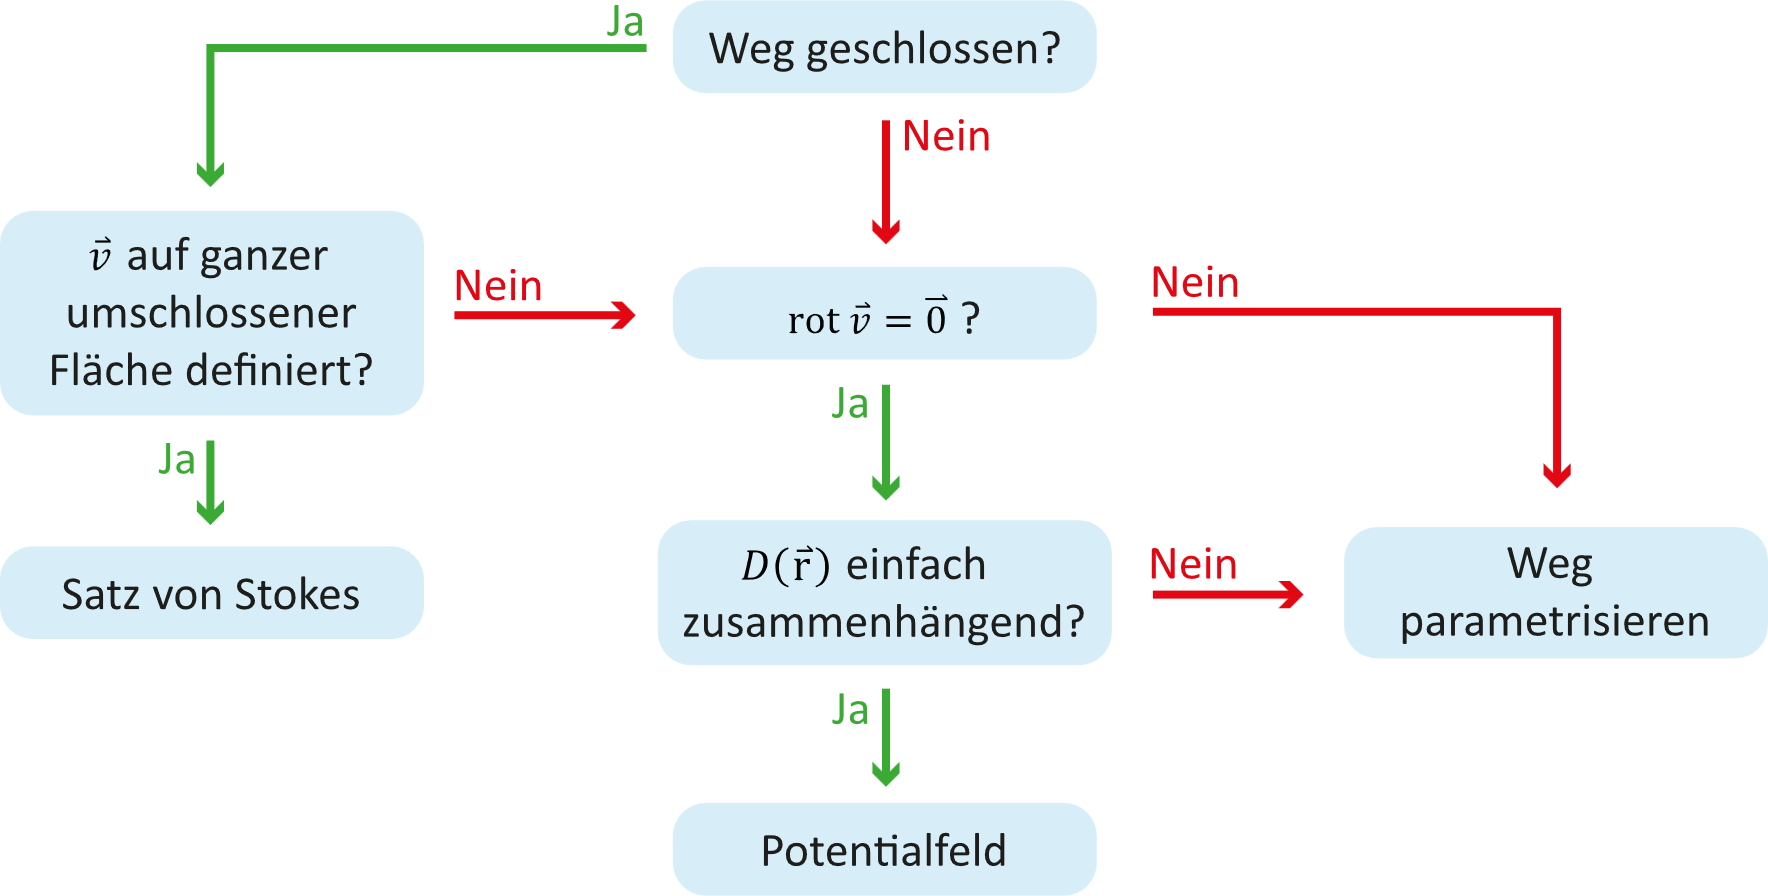
\includegraphics[width=\linewidth,keepaspectratio]{graphics/media/stokes_skizze.png}
\end{formulabox}

\SubsectionBar{Konservative Vektorfelder}
Ein Vektorfeld ist \ZSFkeyword{konservativ}, wenn die Arbeit aller m\"oglichen Wege zwischen zwei Punkten gleich ist, unabh\"angig vom gew\"ahlten Weg.
Dies trifft zu, wenn entweder:
\begin{enumerate}
    \item Die Arbeit entlang aller geschlossenen Wege ist $\displaystyle \oint \vec v\,d\vec r=0$
    \item Oder das Vektorfeld ein \ZSFkeyword{Potentialfeld} ist
\end{enumerate}

Ein \ZSFkeyword{Potentialfeld} ist ein Vektorfeld der Form $\vec v=\grad(f)$ mit Potential $f$.
Bei Potentialfeldern gilt:
\begin{enumerate}
    \item Seien $P$ und $Q$ zwei Punkte, dann $W=f(Q)-f(P)$
    \item Potentialfelder sind wirbelfrei: $\rot\,\vec v=\vec 0$
\end{enumerate}

\ZSFdanger{Achtung:} Wirbelfreie Vektorfelder sind umgekehrt nur dann Potentialfelder, wenn $D(\vec v)$ \ZSFkeyword{einfach zusammenh\"angend} ist.

\textVorBox{Eine Menge $M$ ist \ZSFkeyword{einfach zusammenh\"angend}, wenn sich alle Wege in $M$ auf einen Punkt zusammenziehen lassen, ohne dass $M$ verlassen werden muss:}
\begin{fulltablebox}{Z{0.2} | Y{1.8}}
    $\checkmark$ & $\R^2$, $\R^3$, $\R^3\setminus\{\text{Punkt}\}$, Kugeloberfl\"ache, $\R^3\setminus\{\text{gef\"ullte Kugel}\}$, konvexer gef\"ullter K\"orper \\ \hline
    \ZSFrowColor
    $\times$ & $\R^3\setminus\{\text{Gerade}\}$, Torus, $\R^2\setminus\{\text{Punkt}\}$
\end{fulltablebox}

\textVorBox{\ZSFdanger{Achtung:} F\"ur ein Potentialfeld gilt stets $\rot\,\vec v=\vec 0$. Umgekehrt folgt aus $\rot\,\vec v=\vec 0$ nur bei einfach zusammenh\"angendem $D(\vec v)$ wieder ein Potentialfeld.}
\begin{formulabox}
    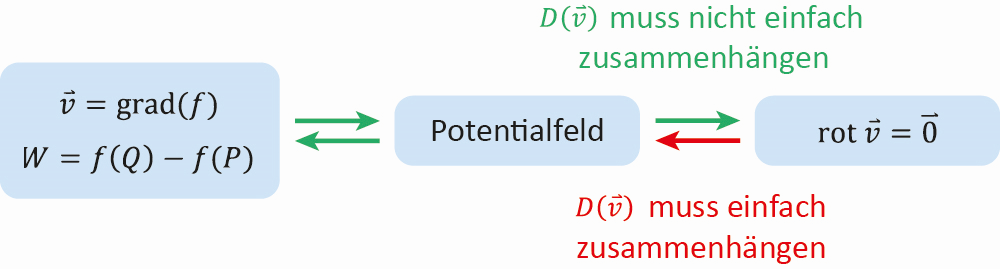
\includegraphics[width=\linewidth,keepaspectratio]{graphics/media/potentialfeld_schema.png}
\end{formulabox}
